\documentclass[handout, 10pt]{beamer}

%\usepackage[backend=bibtex,firstinits=true,style=verbose-inote,citestyle=authortitle]{biblatex}
\usepackage{bm}
\usepackage{graphicx}
\usepackage{subcaption}
\usepackage{amsmath}
\usepackage{makecell}
\usepackage{filecontents}
\usepackage{biblatex}
\newcommand{\expect}[2][]{
\ifthenelse{\equal{#1}{}}{
\mathbb{E}\left[#2\right]
}{
\underset{#1}{\mathbb{E}}\left[#2\right]
}}

\newcommand{\cov}[2][]{
\ifthenelse{\equal{#1}{}}{
\text{Cov}\left[#2\right]
}{
\underset{#1}{\text{Cov}}\left[#2\right]
}}


\newcommand{\var}[2][]{
\ifthenelse{\equal{#1}{}}{
\text{Var}[#2]
}{
\underset{#1}{\text{Var}}[#2]
}}

\newcommand{\loss}[2][]{
\ifthenelse{\equal{#1}{}}{
\mathcal{L}(#2)
}{
\mathcal{L}_{#1}(#2)
}}

\newcommand{\kl}[2]{
\text{D}_\text{KL}[#1 \parallel #2]
}

\newcommand{\R}{\mathbb{R}}
%\newcommand{\Prob}{\mathbb{P}}

\newcommand{\1}[1]{\mathds{1}\{#1\}}


%\usecolortheme{dolphin}
\setbeamertemplate{navigation symbols}{}
\setbeamertemplate{section in toc}{\inserttocsectionnumber.~\inserttocsection}


\title{Normalized and Geometry-Aware Self-Attention Network for Image Captioning}
%\subtitle{}
%\author{Ivan Skorokhodov}
%\date{}
%\logo{
\includegraphics[height=1cm]{images/ipavlov-logo.png}}

\newcommand{\citepaper}[1]{\citetitle{#1} by \citeauthor{#1}}

%\graphicspath{{./images}}

%\usetheme{lucid}
\begin{document}

\begin{frame}
    \titlepage
\end{frame}

\begin{frame}
\frametitle{Self-Attention Networks for Image Captioning}

\begin{columns}
\begin{column}{0.5\textwidth}
\begin{itemize}
    \item\pause Take a usual Transformer model for machine translation;
    \item\pause Use a pretrained Faster-RCNN model to extract objects and pass objects' features as an input to the encoder.
    \item\pause Do not use positional embeddings for encoder
\end{itemize}
\end{column}
\begin{column}{0.5\textwidth}
\pause
\begin{figure}
    \centering
    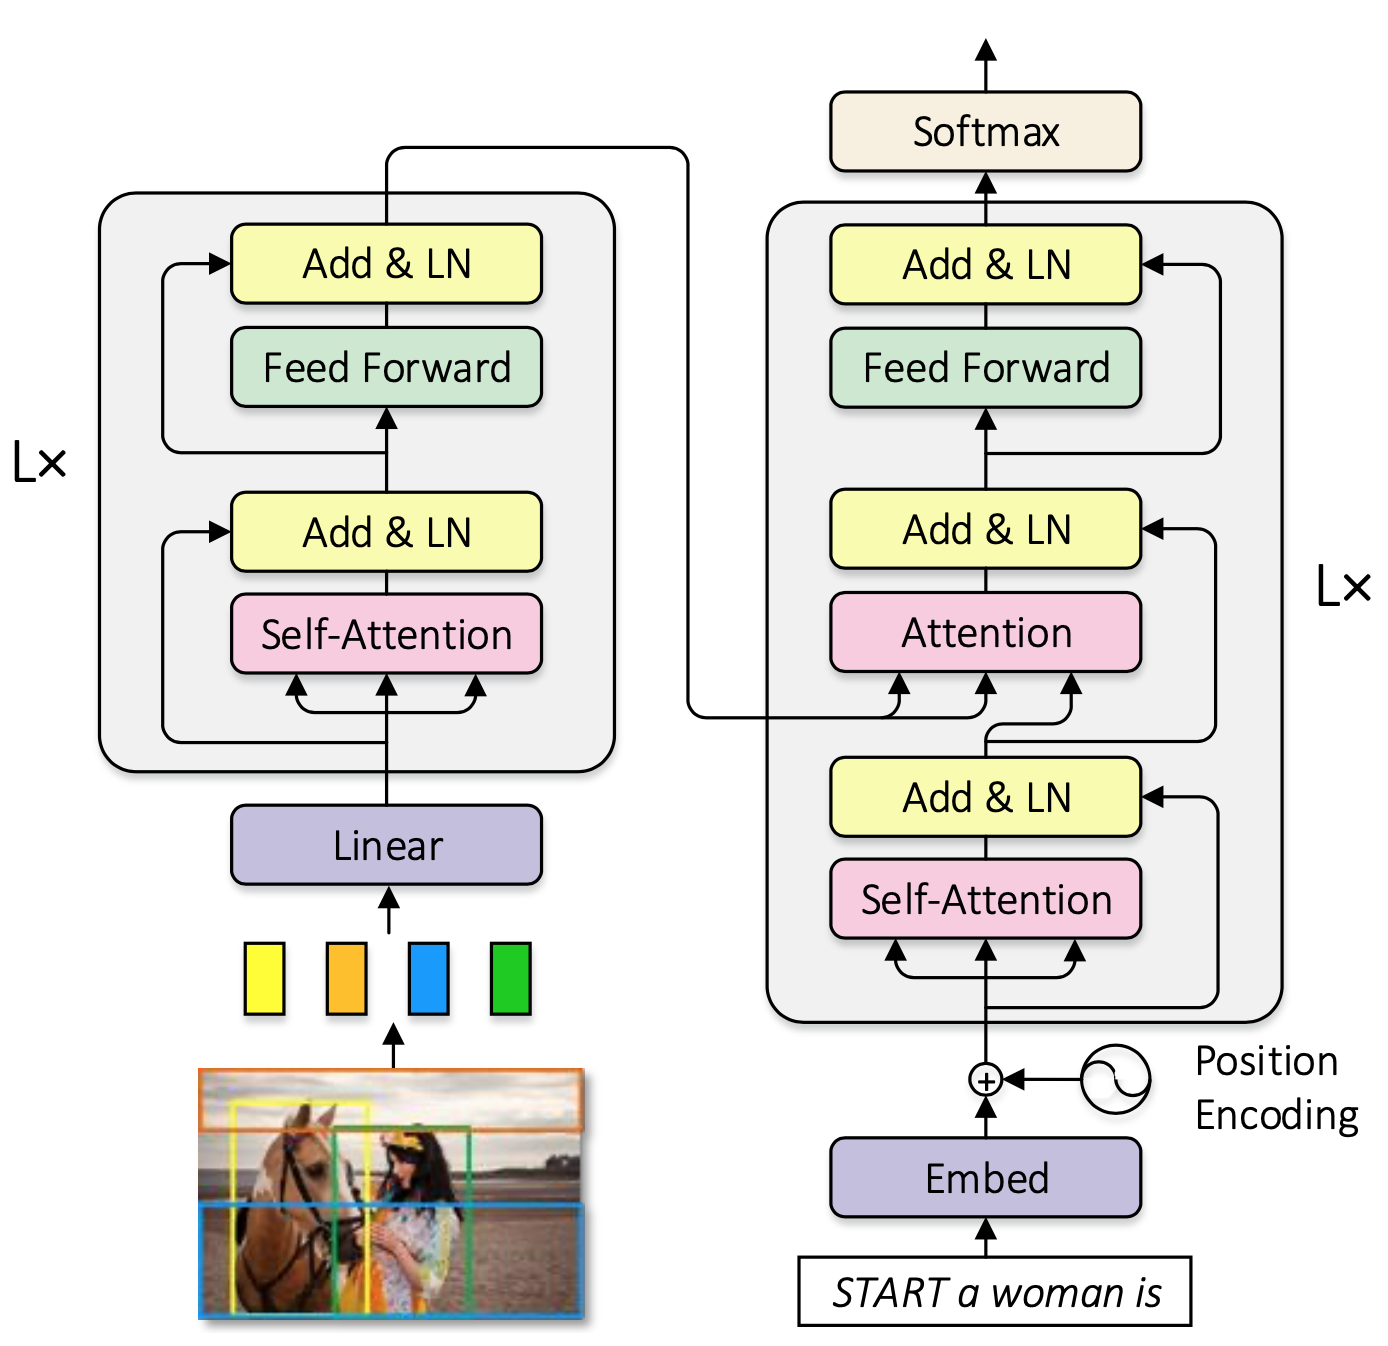
\includegraphics[width=\textwidth]{images/san.png}
\end{figure}
\end{column}
\end{columns}

\end{frame}

\begin{frame}
    \frametitle{Normalization for an attention mechanism (N-SAN)}
    \begin{itemize}
        \item Attention weights are calculated as:
        
\begin{equation}
\begin{aligned}
S &=\operatorname{Softmax}\left(Q K^{\top}\right) \\
&=\operatorname{Softmax}\left(\left(X W_{Q}\right) \cdot\left(W_{K}^{\top} X^{\top}\right)\right)
\end{aligned}
\end{equation}
        
        \item The paper shows that it is beneficial to apply Instance Normalization to matrix $Q$:

\begin{equation}
\begin{aligned}
\hat{x}_{b t c} &=\frac{x_{b t c}-\mu_{b c}}{\sqrt{\sigma_{b c}^{2}+\epsilon}} \\
\mu_{b c}=\frac{1}{T} \sum_{t=1}^{T} x_{b t c}, & \sigma_{b c}^{2}=\frac{1}{T} \sum_{t=1}^{T}\left(x_{b t c}-\mu_{b c}\right)^{2}
\end{aligned}
\end{equation}

    \item i.e. we normalize each sample independently across time dimension;
    \end{itemize}
\end{frame}

\begin{frame}
    \frametitle{Incorporating geometry information (G-SAN)}
    \begin{itemize}
        \item What if we mix positional information into attention calculation?

\begin{equation}
\begin{aligned}
S &=\operatorname{Softmax}\left(Q K^{\top} + \phi(Q', K', G) \right)
\end{aligned}
\end{equation}
    \item\pause Matrix $G$ carries some non-trivial information about objects geometry.
    \item\pause Here $\phi$ is a matrix of $\phi_{ij}(Q'_i, K'_j, G_{ij})$ 
    \item\pause $\phi_{ij}$ is a one-layer NN on top of combinations of $Q'_i, K'_j$ and $G_{ij}$.
    \item\pause Authors consider different variants to combine three ingredients together.
    \item\pause We compute $G_{i j}=\operatorname{ReLU}\left(\mathrm{FC}\left(\mathbf{f}_{i j}^{g}\right)\right)$ from $\mathbf{f}_{i j}^{g}$ which is a 4-dimensional vector of:
\begin{equation}
\mathbf{f}_{i j}^{g}=\left(\log \left(\frac{\left|x_{i}-x_{j}\right|}{w_{i}}\right), \log \left(\frac{\left|y_{i}-y_{j}\right|}{h_{i}}\right), \log \left(\frac{w_{i}}{w_{j}}\right), \log \left(\frac{h_{i}}{h_{j}}\right)\right)^{T-}
\end{equation}
    \end{itemize}
\end{frame}

\begin{frame}
    \frametitle{Some results and considerations}
    \begin{itemize}
        \item\pause Authors test an NG-SAN model on 2 tasks: image captioning, video question answering;
        \item\pause Authors additionally test an N-SAN model on 2 tasks: video captioning, machine translation.
        \item\pause Almost all the scores are improved somewhat marginally: +0.1-0.3 absolute points (0.2-0.7\% of relative improvement). But seems like it is a lot for image captioning.
        \item\pause Authors do not provide stds of the runs which would be very helpful.
    \end{itemize}
\end{frame}

\end{document}
